%----------------------------------------------------------------------------------------
%	PACKAGES AND OTHER DOCUMENT CONFIGURATIONS
%----------------------------------------------------------------------------------------

\documentclass[final]{beamer}

\usepackage[scale=0.78, size=a1]{beamerposter} % Use the beamerposter package for laying out the poster

\usetheme{confposter} % Use the confposter theme supplied with this template

\setbeamercolor{block title}{fg=dblue,bg=white} % Colors of the block titles
\setbeamercolor{block body}{fg=black,bg=white} % Colors of the body of blocks
\setbeamercolor{block alerted title}{fg=white,bg=dblue!70} % Colors of the highlighted block titles
\setbeamercolor{block alerted body}{fg=black,bg=white} % Colors of the body of highlighted blocks
% Many more colors are available for use in beamerthemeconfposter.sty

%-----------------------------------------------------------
% Define the column widths and overall poster size
% To set effective sepwid, onecolwid and twocolwid values, first choose how many columns you want and how much separation you want between columns
% In this template, the separation width chosen is 0.024 of the paper width and a 4-column layout
% onecolwid should therefore be (1-(# of columns+1)*sepwid)/# of columns e.g. (1-(4+1)*0.024)/4 = 0.22
% Set twocolwid to be (2*onecolwid)+sepwid = 0.464
% Set threecolwid to be (3*onecolwid)+2*sepwid = 0.708

\newlength{\sepwid}
\newlength{\onecolwid}
\newlength{\twocolwid}
\newlength{\threecolwid}
\setlength{\paperwidth}{33.11in} % A0 width: 46.8in
\setlength{\paperheight}{23.39in} % A0 height: 33.1in
\setlength{\sepwid}{0.00\paperwidth} % Separation width (white space) between columns
\setlength{\onecolwid}{0.20\paperwidth} % Width of one column
\setlength{\twocolwid}{0.464\paperwidth} % Width of two columns
\setlength{\threecolwid}{0.708\paperwidth} % Width of three columns
\setlength{\topmargin}{-0.8in} % Reduce the top margin size
%-----------------------------------------------------------

\usepackage{graphicx}  % Required for including images

\usepackage{booktabs} % Top and bottom rules for tables

\usepackage{exscale}

%----------------------------------------------------------------------------------------
%	TITLE SECTION 
%----------------------------------------------------------------------------------------



\title{Designing Neural Network Hardware Accelerators \\[0.1in] Using Deep Gaussian Processes
}

\author{M. Havasi, \\ \vspace{0.1in} Supervisor: Dr. J. M. Hernandez-Lobato} % Author(s)

\institute{June, 2017} % Institution(s)

%----------------------------------------------------------------------------------------

\begin{document}


\addtobeamertemplate{block end}{}{\vspace*{1ex}} % White space under blocks
\addtobeamertemplate{block alerted end}{}{\vspace*{1ex}} % White space under highlighted (alert) blocks

\setlength{\belowcaptionskip}{1ex} % White space under figures
\setlength\belowdisplayshortskip{1ex} % White space under equations

\begin{frame}[t] % The whole poster is enclosed in one beamer frame

\begin{columns}[t] % The whole poster consists of three major columns, the second of which is split into two columns twice - the [t] option aligns each column's content to the top

\begin{column}{\sepwid}\end{column} % Empty spacer column

\begin{column}{\onecolwid} % The first column

%----------------------------------------------------------------------------------------
%	INTRODUCTION
%----------------------------------------------------------------------------------------

\begin{block}{Introduction}

In this project, Bayesian optimization methods are employed in a hardware design setting where simulation of a given hardware configuration can be computationally very expensive. An additional twist is that there are multiple objective functions, the power consumption and the accuracy, to balance against each other.
\end{block}

%------------------------------------------------


\begin{block}{Deep Gaussian Processes}

Deep Gaussian processes (DGPs) are multi-layer hierarchical generalizations of Gaussian processes
(GPs) and are formally equivalent to neural networks with multiple, infinitely wide hidden
layers.

$$p(f_l|\theta_l)=\mathcal{GP}(f_l; \boldsymbol 0, \boldsymbol K_l)$$

$$p(\boldsymbol h_l|f_l, \boldsymbol h_{l-1}, \sigma_l^2)=\prod_n\mathcal{N}(h_{l,n};f_l(h_{l-1, n}), \sigma_l^2)$$

Approximate Inference is attained using Expectation Propagation.

$$log(\boldsymbol y|\alpha)\approx \mathcal{F}(\alpha)=\phi(\theta)-\phi(\theta_{prior}) + \sum_{n=1}^N log \tilde{Z}_n$$

$$log \tilde{Z}_n = log Z_n + \phi(\theta^{\setminus n}) - \phi(\theta)$$

\end{block}
\begin{figure}
\includegraphics[width=\linewidth]{dgp.PNG}
\end{figure}

%----------------------------------------------------------------------------------------

\end{column} % End of the first column

\begin{column}{\sepwid}\end{column} % Empty spacer column

\begin{column}{\twocolwid} % Begin a column which is two columns wide (column 2)

\begin{columns}[t,totalwidth=\twocolwid] % Split up the two columns wide column

\begin{column}{\onecolwid}\vspace{-.6in} % The first column within column 2 (column 2.1)

%----------------------------------------------------------------------------------------
%	MATERIALS
%----------------------------------------------------------------------------------------

\begin{block}{Multiobjective Optimization}

The goal is to find the set of optimal configurations that are not outperformed in both objective functions. These points are called the Pareto front.

We are using an acquisition function to determine where the next evaluation will take place. The aim of this heuristic function is to determine which evaluations will lead to the best Pareto front approximation.

\end{block}

%----------------------------------------------------------------------------------------

\end{column} % End of column 2.1

\begin{column}{\onecolwid}\vspace{-.6in} % The second column within column 2 (column 2.2)

%----------------------------------------------------------------------------------------
%	METHODS
%----------------------------------------------------------------------------------------

\begin{block}{Acquisition function}

Our aquisition function is S-Metric Selection-based Efficient Global Optimization (SMSego) which aims to maximize the hypervolume of the Pareto front.

It uses the lower confidence bound (LCB) for predicted values $\tilde{y}$ and uncertainties $\tilde{s}$: $$\tilde{y}_{pot} = \tilde{y} - \alpha \tilde{s}$$

If the potential is dominated by a Pareto point then a penalty is applied along the non-$\epsilon$-dominated dimensions.


\end{block}

%----------------------------------------------------------------------------------------

\end{column} % End of column 2.2

\end{columns} % End of the split of column 2 - any content after this will now take up 2 columns width

%----------------------------------------------------------------------------------------
%	IMPORTANT RESULT
%----------------------------------------------------------------------------------------

\begin{alertblock}{2D Example}

\begin{figure}
\centering
\begin{minipage}{.33\textwidth}
  \centering
  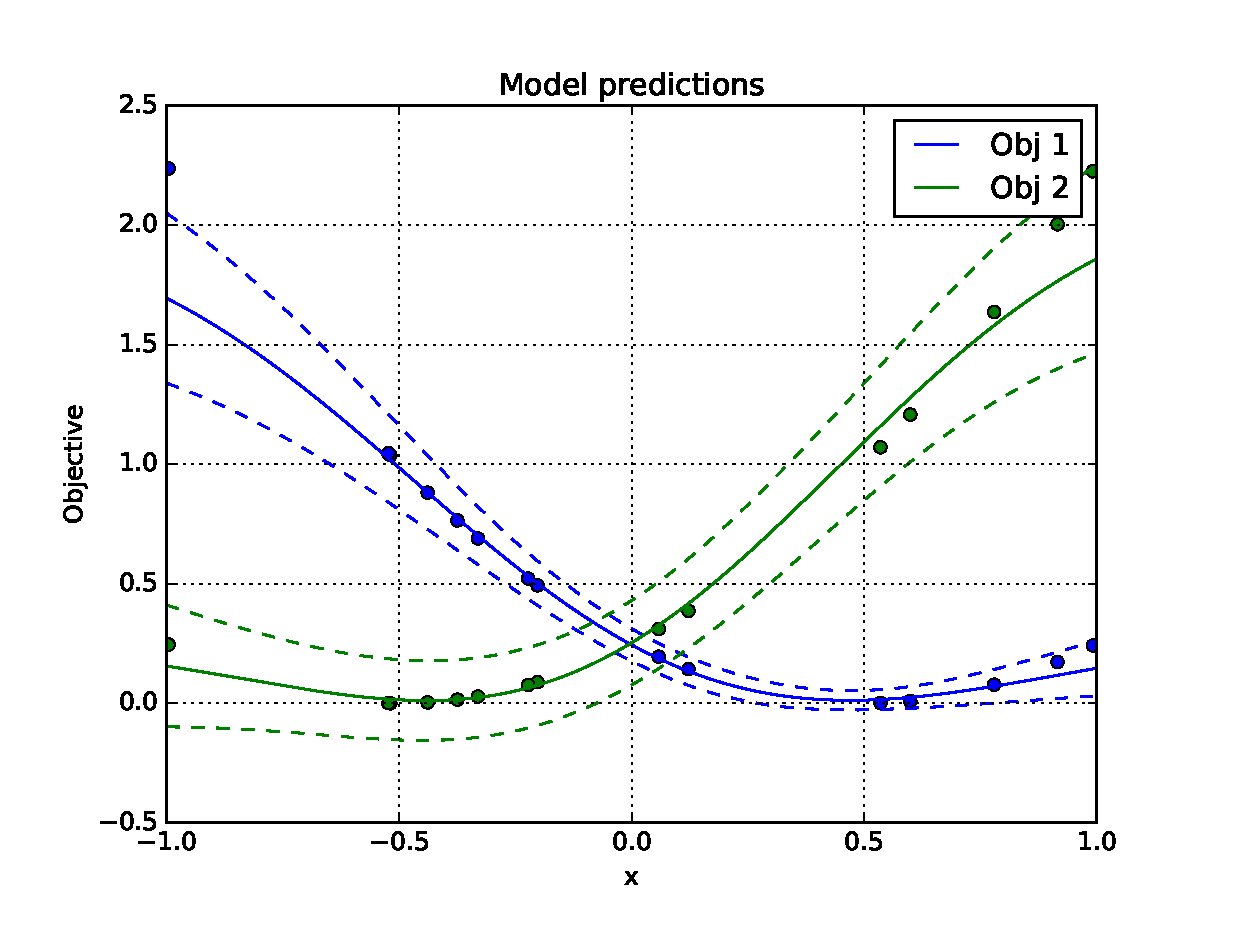
\includegraphics[width=\linewidth]{optimizer/model.eps}
\end{minipage}%
\begin{minipage}{.33\textwidth}
  \centering
  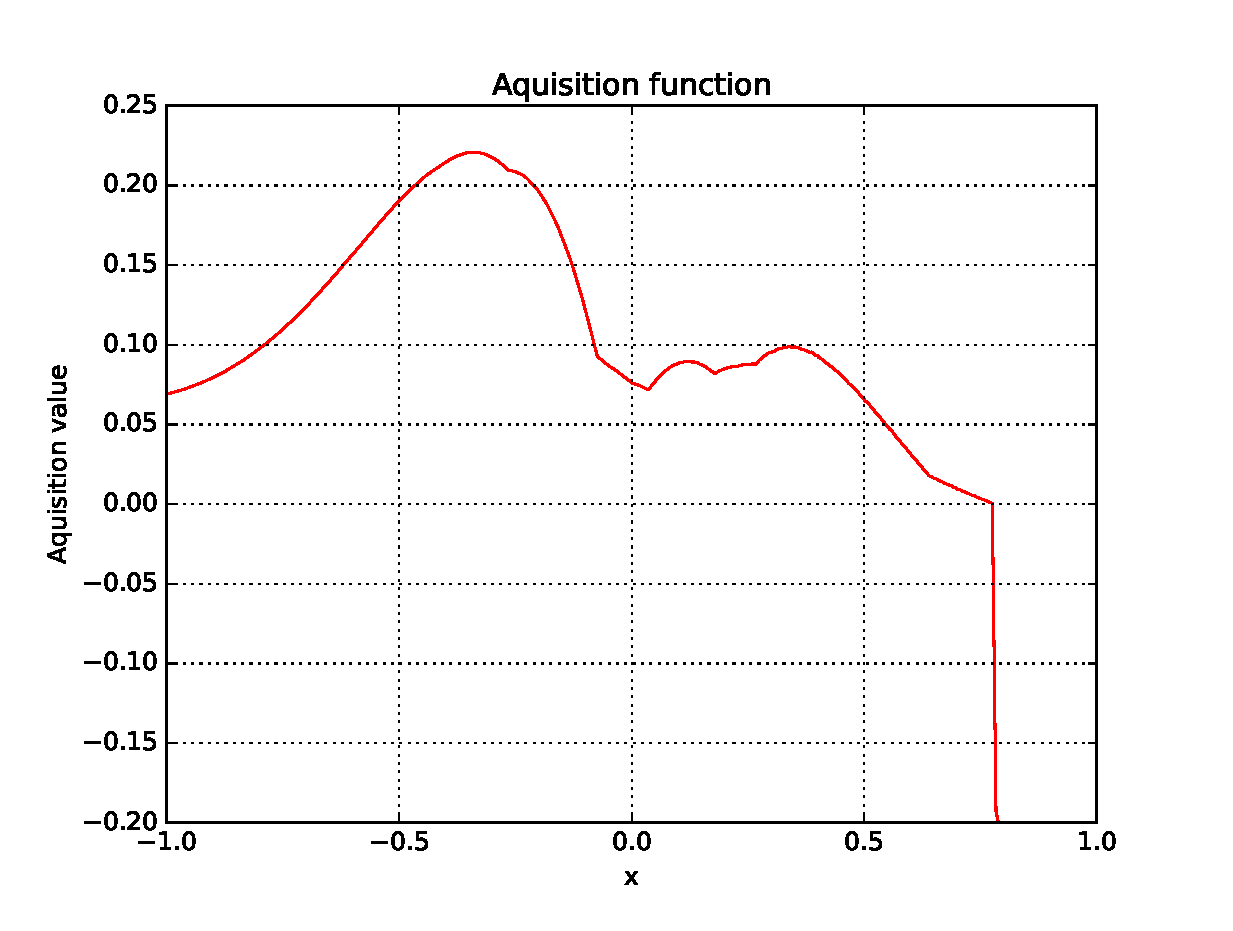
\includegraphics[width=\linewidth]{optimizer/aquisition.eps}
\end{minipage}
\begin{minipage}{.33\textwidth}
  \centering
  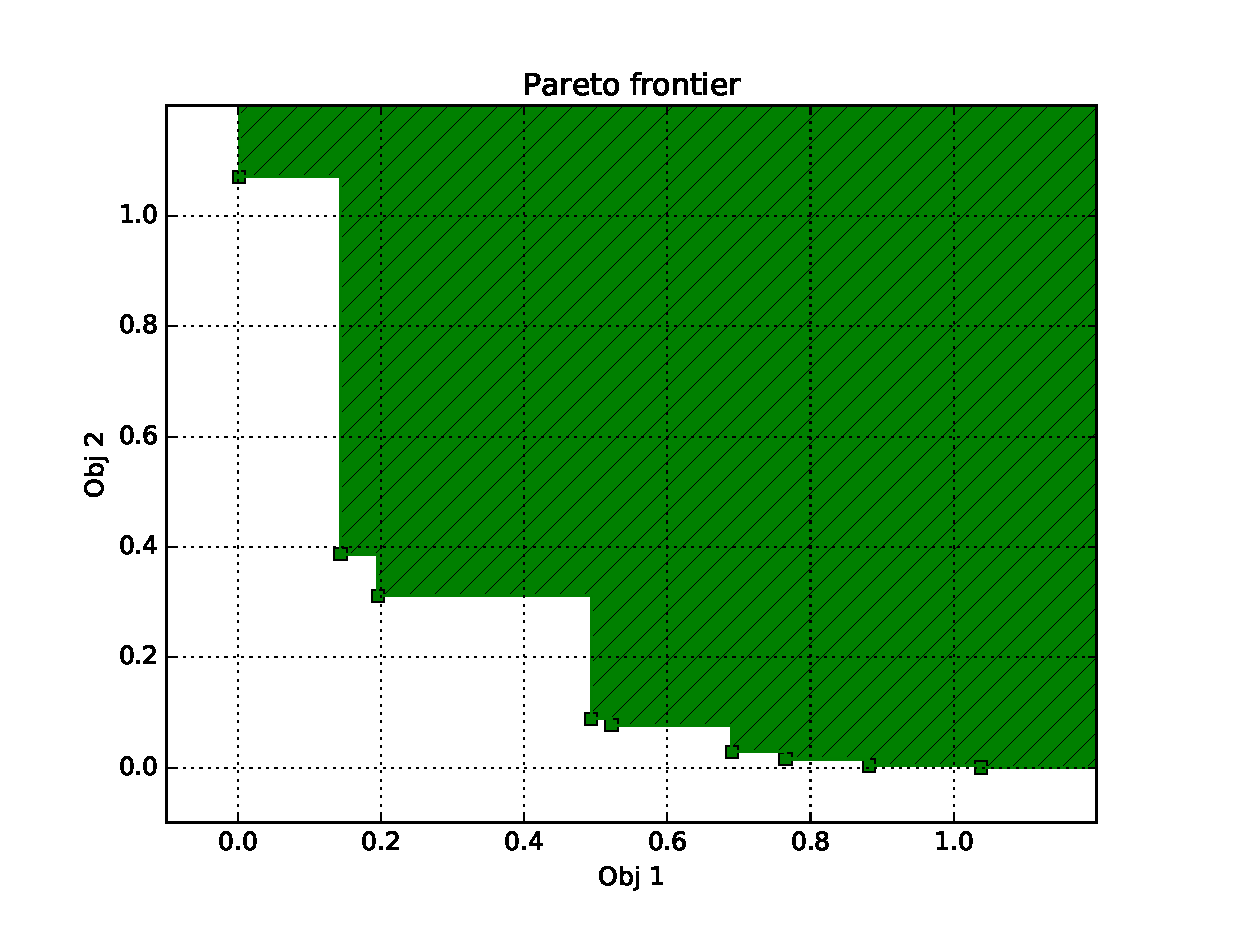
\includegraphics[width=\linewidth]{optimizer/pareto.eps}
\end{minipage}
\end{figure}

\end{alertblock} 

%----------------------------------------------------------------------------------------
%	RESULTS
%----------------------------------------------------------------------------------------

\begin{block}{Initial Results}

This is an example run on real data draw from neural network hardware accelerators. The inputs were 13 dimensional configurations and the two objectives were power consumption and prediction accuracy.

\begin{figure}
\centering
\begin{minipage}{.5\textwidth}
  \centering
  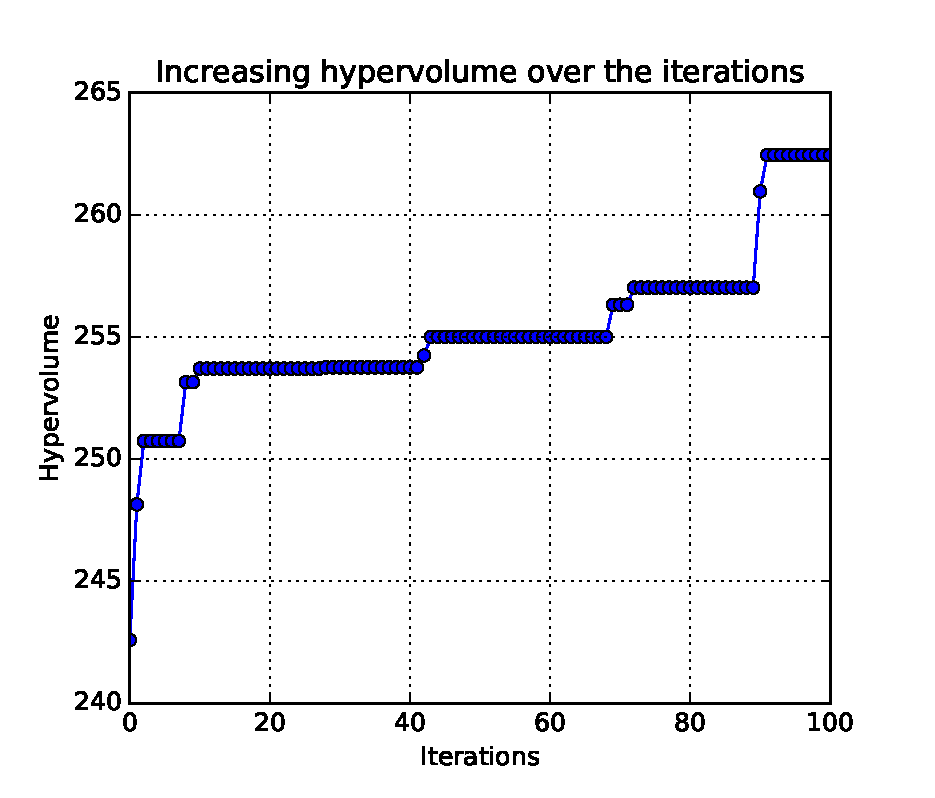
\includegraphics[width=\linewidth]{data/curve.eps}
\end{minipage}%
\begin{minipage}{.5\textwidth}
  \centering
  \includegraphics[width=\linewidth]{data/evals.eps}
\end{minipage}
\end{figure}

\end{block}

%----------------------------------------------------------------------------------------

\end{column} % End of the second column

\begin{column}{\sepwid}\end{column} % Empty spacer column

\begin{column}{\onecolwid} % The third column

%----------------------------------------------------------------------------------------
%	CONCLUSION
%----------------------------------------------------------------------------------------

\begin{block}{Applications}

The methodology is applicable in any setting where evaluating the objective function is costly and there are multiple objectives to balance against each other.

There is a wide range of applications such as:

\begin{itemize}
\item Optimizing hardware configurations
\item Optimizing neural-network hyperparameters
\end{itemize}

\end{block}

%----------------------------------------------------------------------------------------
%	ADDITIONAL INFORMATION
%----------------------------------------------------------------------------------------

\begin{block}{Further Work}

During the remaining time of this project, we will focus on collecting more data. We want to establish baselines using existing methods and evaluate the relative performance.

We are also considering extensions that will speed up the otherwise expensive ($O(NLK^2)$) runtime.

\end{block}

%----------------------------------------------------------------------------------------
%	REFERENCES
%----------------------------------------------------------------------------------------

\setbeamercolor{block alerted title}{fg=black,bg=norange} % Change the alert block title colors
\setbeamercolor{block alerted body}{fg=black,bg=white} % Change the alert block body colors

\begin{alertblock}{References}

\small
\begin{thebibliography}{9}
\bibitem{dgps} 
Bui T. D., Hern\'andez-Lobato J. M., Li Y., Hern\'andez-Lobato D. and Turner R. E. Deep
\textit{Gaussian Processes for Regression using Approximate Expectation Propagation}, In ICML,
2016.
 
\bibitem{smsego} 
W. Ponweiser, T. Wagner, D. Biermann, and M. Vincze,  
\textit{Multiobjective optimization on a limited budget of evaluations using model-assisted s-metric selection} in Proc. Parallel Problem Solving from Nature (PPSN X) , Dortmund, Germany, Sept. 2008, pp. 784–794. 

\bibitem{hardware} 
Hern\'andez-Lobato J. M., Gelbart M. A., Reagen B., Adolf R., Hern\'andez-Lobato D., What-
mough P., Brooks D., Wei G.-Y. and Adams R. P. \textit{Designing Neural Network Hardware
Accelerators with Decoupled Objective Evaluations}, In NIPS Workshop on Bayesian Opti-
mization, Barcelona, Spain, 2016.

\bibitem{acc}
Reagen B., Whatmough P. Adolf R., Rama S., Lee H., Lee S., Hern\'andez-Lobato J. M., Wei
G. Y. and Brooks D. \textit{Minerva: Enabling Low-Power, High-Accuracy Deep Neural Network
Accelerators}, In ISCA, 2016.
\end{thebibliography}

\end{alertblock}


%----------------------------------------------------------------------------------------

\end{column} % End of the third column

\end{columns} % End of all the columns in the poster

\end{frame} % End of the enclosing frame

\end{document}
